\documentclass[12pt, titlepage]{article}

\usepackage{booktabs}
\usepackage{tabularx}
\usepackage{hyperref}
\hypersetup{
    colorlinks,
    citecolor=black,
    filecolor=black,
    linkcolor=red,
    urlcolor=blue
}
\usepackage[round]{natbib}

\usepackage{amsmath, amsfonts}
\usepackage[margin=1in]{geometry}
\usepackage{amssymb}
\usepackage{amsthm}
\usepackage{amsmath}
\usepackage{multirow}
\usepackage{verbatim}
\usepackage{listings}
\usepackage{color}
\usepackage{hyperref}
\usepackage{blindtext}
\usepackage{cancel}
\usepackage{float}
\usepackage{enumitem}
\usepackage{graphicx}
\usepackage{makecell}
\usepackage{longtable}

\usepackage[table]{xcolor}
\setlength{\tabcolsep}{18pt}
\renewcommand{\arraystretch}{1.5}
\renewcommand{\labelenumi}{\theenumi.}
\renewcommand{\labelenumii}{\theenumii.}
\renewcommand{\labelenumiii}{\theenumiii.}
\newcommand{\be}{\begin{enumerate}}
\newcommand{\ee}{\end{enumerate}}
\newcommand{\bi}{\begin{itemize}}
\newcommand{\ei}{\end{itemize}}
\newcommand{\bc}{\begin{center}}
\newcommand{\ec}{\end{center}}
\newcommand{\bv}{\begin{verbatim}}
\newcommand{\ev}{\end{verbatim}}
\newcommand{\ba}{\begin{align*}}
\newcommand{\ea}{\end{align*}}
\newcommand{\beq}{\begin{equation*}}
\newcommand{\eeq}{\end{equation*}}
\newcommand{\bs}{\begin{split}}
\newcommand{\es}{\end{split}}
\newcommand{\mname}[1]{\mbox{\sf #1}}
\newcommand{\pnote}[1]{{\langle \text{#1} \rangle}}
\renewcommand{\labelenumii}{\theenumii.}


\title{Software Requirements Specification\\ASLingo Application}

\author{Team 15, ASLingo
		\\ Andrew Kil
		\\ Cassidy Baldin
		\\ Edward Zhuang
		\\ Jeremy Langner
		\\ Stanley Chan
}

\date{\today}

%% Comments

\usepackage{color}

\newif\ifcomments\commentstrue %displays comments
%\newif\ifcomments\commentsfalse %so that comments do not display

\ifcomments
\newcommand{\authornote}[3]{\textcolor{#1}{[#3 ---#2]}}
\newcommand{\todo}[1]{\textcolor{red}{[TODO: #1]}}
\else
\newcommand{\authornote}[3]{}
\newcommand{\todo}[1]{}
\fi

\newcommand{\wss}[1]{\authornote{blue}{SS}{#1}} 
\newcommand{\plt}[1]{\authornote{magenta}{TPLT}{#1}} %For explanation of the template
\newcommand{\an}[1]{\authornote{cyan}{Author}{#1}}

%% Common Parts

\newcommand{\progname}{Software Engineering} % PUT YOUR PROGRAM NAME HERE
\newcommand{\authname}{Team 15, ASLingo
\\ Andrew Kil
\\ Cassidy Baldin
\\ Edward Zhuang
\\ Jeremy Langner
\\ Stanley Chan} % AUTHOR NAMES                  

\usepackage{hyperref}
    \hypersetup{colorlinks=true, linkcolor=blue, citecolor=blue, filecolor=blue,
                urlcolor=blue, unicode=false}
    \urlstyle{same}
                                


\begin{document}

\maketitle

\pagenumbering{roman}
\tableofcontents
\listoftables
\listoffigures

\newpage

\begin{longtable}{| c | p{3cm} | p{6.5cm} |}
\caption{Revision History} \\
\hline {\bf Date} & {\bf Developers} & {\bf Change}\\
\hline
September 25, 2023 & All team members & Initial draft, added some functional requirements \\
September 26, 2023 & Andrew Kil & Added constraints and naming conventions \\
September 26, 2023 & Cassidy Baldin & Added some functional and non-functional requirements \\
September 27, 2023 & Jeremy Langner & Added some points to section 4 Project Issues \\
September 28, 2023 & Cassidy Baldin & Added NFR tables, some rationales for NFRs \\
September 28, 2023 & Andrew Kil & Added abbreviations and assumptions \\
September 28, 2023 & Stanley Chan & Added scope and context of work, some work partitioning events \\
September 28, 2023 & Edward Zhuang & Added to Section 4 and some FR rationales \\
October 2, 2023 & Cassidy Baldin & Edited Section 3 requirements, finished all rationales \\
October 4, 2023 & Stanley Chan & Added individual product use cases, updated work partitioning \\
October 4, 2023 & Edward Zhuang & Edited Section 4 according to meeting with MSLC, and added response to one reflection question \\
October 6, 2023 & Cassidy Baldin & Added fit criterion, fixed formatting, added reflection \\
October 6, 2023 & Stanley Chan & Added individual reflection \\
October 6, 2023 & Jeremy Langner & Added personal reflection response and general reflection question 3. \\
October 6, 2023 & Andrew Kil & Added personal reflection response\\
October 19, 2023 & Cassidy Baldin & Revised aspects of the SRS after given peer review feedback. \\
November 1, 2023 & Jeremy Langner & Added in FR, Use case for reseting password credentials. Switched traceability matrix to table instead of jpeg\\
Jan 23, 2024 & Cassidy Baldin & Addressed git issue \#49 regarding NFRT2 - PT3 and PR3 \\
\bottomrule
\end{longtable}

\newpage

\pagenumbering{arabic}

This document describes the requirements for ASLingo. The template for the Software
Requirements Specification (SRS) is a subset of the Volere
template \textit{Robertson And Robertson (2012)}.  Subsections \textit{Clients} and \textit{Customers} were removed due to not having any such dependents.

\section{Project Drivers}

\subsection{The Purpose of the Project}

Learning a new language can be an arduous task that only gets more challenging
with age, as individuals may find it difficult to dedicate time and effort to
it. American Sign Language (ASL) is particularly hard due to its visual and
gestural nature, which is not found in other, verbal languages. The purpose of this project is
to ease that challenge by providing an online, easy-to-access web platform for
individuals to learn new signs and test their comprehension at their own pace
in a fun, interactive manner. Focusing in on consistent effort and continuous
feedback, ASLingo provides real-time guidance to ensure users stay on track to
achieving their goals of learning ASL.

\subsection{The Stakeholders}

 The stakeholders for this project include those who use sign language as their primary mode of communication in daily life as well as those who have an interest in learning ASL, as one of the main objectives of this project is to help people to learn ASL easier. This would naturally expand outward towards secondary users of this application which may be educators who wish to promote the learning of ASL to their respective institutions. The objectives of the stakeholders for this project should be the ability to learn ASL more effectively as they will not only be able to recognize what signs mean, but will be able to practice signing themselves to better their understanding. This therefore should also be an application that is able to be used for both individuals who cannot hear and those who can, as we want to further the understanding of ASL for a wide variety of users with varying differences in abilities. 

% \subsubsection{The Client}
% \subsubsection{The Customers}
% \subsubsection{Other Stakeholders}

\subsection{Mandated Constraints}

The project is constrained by the following:

\begin{itemize}
    \item[] \textbf{\textit{The Project Expenses Cannot Exceed \$750}}
    \begin{itemize}
        \item The project cannot be bought or be a `ready-made' solution, and any cost incurred must be minimized to ensure cost-efficiency.
    \end{itemize}
    \item[] \textbf{\textit{Test Only a Subset of the Most Commonly Used Phrases of ASL}}
    \begin{itemize}
        \item The project in the long-term would encompass the entirety of ASL as a whole. But with the given time-constraints, the testable language subset will be limited.
    \end{itemize}
    \item[] \textbf{\textit{The Project Must be Finished by the End of the Academic Year}}
    \begin{itemize}
        \item This is the hard deadline for the project and sets the time constraint that is used to judge the scope of work the project can encompass.
    \end{itemize}
    \item[] \textbf{\textit{Users Should Only Learn from the Provided "On Rails" Approach}}
    \begin{itemize}
        \item Users are only able to learn from the preset programs the project has. The education provided should be taught in a manner with little room misinterpretation. While we attempt to make the learning content as broad as possible, users lack true learning freedom to learn what they want.
    \end{itemize}
\end{itemize}

\subsection{Naming Conventions and Terminology}

\begin{longtable}{| c | p{7cm} |}
\caption{Naming Conventions and Terminology} \\
\hline
\textbf{Term, Abbreviation, or Acronym} & \textbf{Description}\\
\hline
A & Shorthand for Assumption\\
\hline
ASL & Shorthand for American Sign Language. It is a form of sign language primarily used in the US and in parts of Canada\\
\hline
ASLingo & The commercial name for the project\\
\hline
CV & Refers to Computer Vision, the field of technology that involves processing visual input to achieve various means.\\
\hline
CR & Shorthand for 'Cultural Requirements', a subsection of Non-Functional Requirements.\\
\hline
HSR & Shorthand for 'Health and Safety Requirements', a subsection of Non-Functional Requirements.\\
\hline
FR & Shorthand for Functional Requirements\\
\hline
LR & Shorthand for 'Legal Requirements', a subsection of Non-Functional Requirements.\\
\hline
LFR & Shorthand for 'Look and Feel Requirements', a subsection of Non-Functional Requirements.\\
\hline
MSR & Shorthand for 'Maintainability and Support Requirements', a subsection of Non-Functional Requirements.\\
\hline
OER & Shorthand for 'Operational and Environmental Requirements', a subsection of Non-Functional Requirements.\\
\hline
OpenCV & Refers to the Open Computer Vision Library library available for free to developers in order to develop Computer Vision applications.\\
\hline
PR & Shorthand for 'Performance Requirements', a subsection of Non-Functional Requirements.\\
\hline
SR & Shorthand for 'Security Requirements', a subsection of Non-Functional Requirements.\\
\hline
UHR & Shorthand for 'Usability and Humanity Requirements', a subsection of Non-Functional Requirements.\\
\bottomrule
\end{longtable}

\subsection{Relevant Facts and Assumptions}

\begin{enumerate}
    \item The user will always have the camera facing their hands when using the application.
    \begin{itemize}
        \item[] Correct camera angling towards the user's hands is the first condition for the application to work.
    \end{itemize}
    \item The environmental lighting will always be sufficient for joint detection.
    \begin{itemize}
        \item[] Proper lighting is the second condition for the application to work since it cannot properly distinct what the user signs without it.
    \end{itemize}
    \item The user's signs will be within reasonable form of the proper sign, enough to be recognized by the system.
    \begin{itemize}
        \item[] If the user signs are correct but with poor form, the system will have a hard time determining if it is correct.
    \end{itemize}
    \item The user's camera will have the necessary technical requirements to accurately capture the signs displayed by the user.
    \begin{itemize}
        \item[] The user's camera should have the capability of viewing the input of the user, with ample resolution and frame rate.
    \end{itemize}
\end{enumerate}

\section{Functional Requirements}

\subsection{The Scope of the Work and the Product}
The scope of ASLingo can be clearly defined by outlining our primary goals for this product.

\begin{enumerate}
  \item Hand Sign Recognition: Reliably recognize users' hand sign in real-time based on the American Sign Language.
  \item Test Users: Quiz users with sign language based questions.
  \item User Progression: Track a user's sign language learning progression.
  \item Account Management: Store required user information to allow users to create and login to their accounts.
\end{enumerate}

\subsubsection{The Context of the Work}
The following is a context diagram which describes the high-level overview on how the system will be utilized.

\begin{figure}[H]
    \centering
    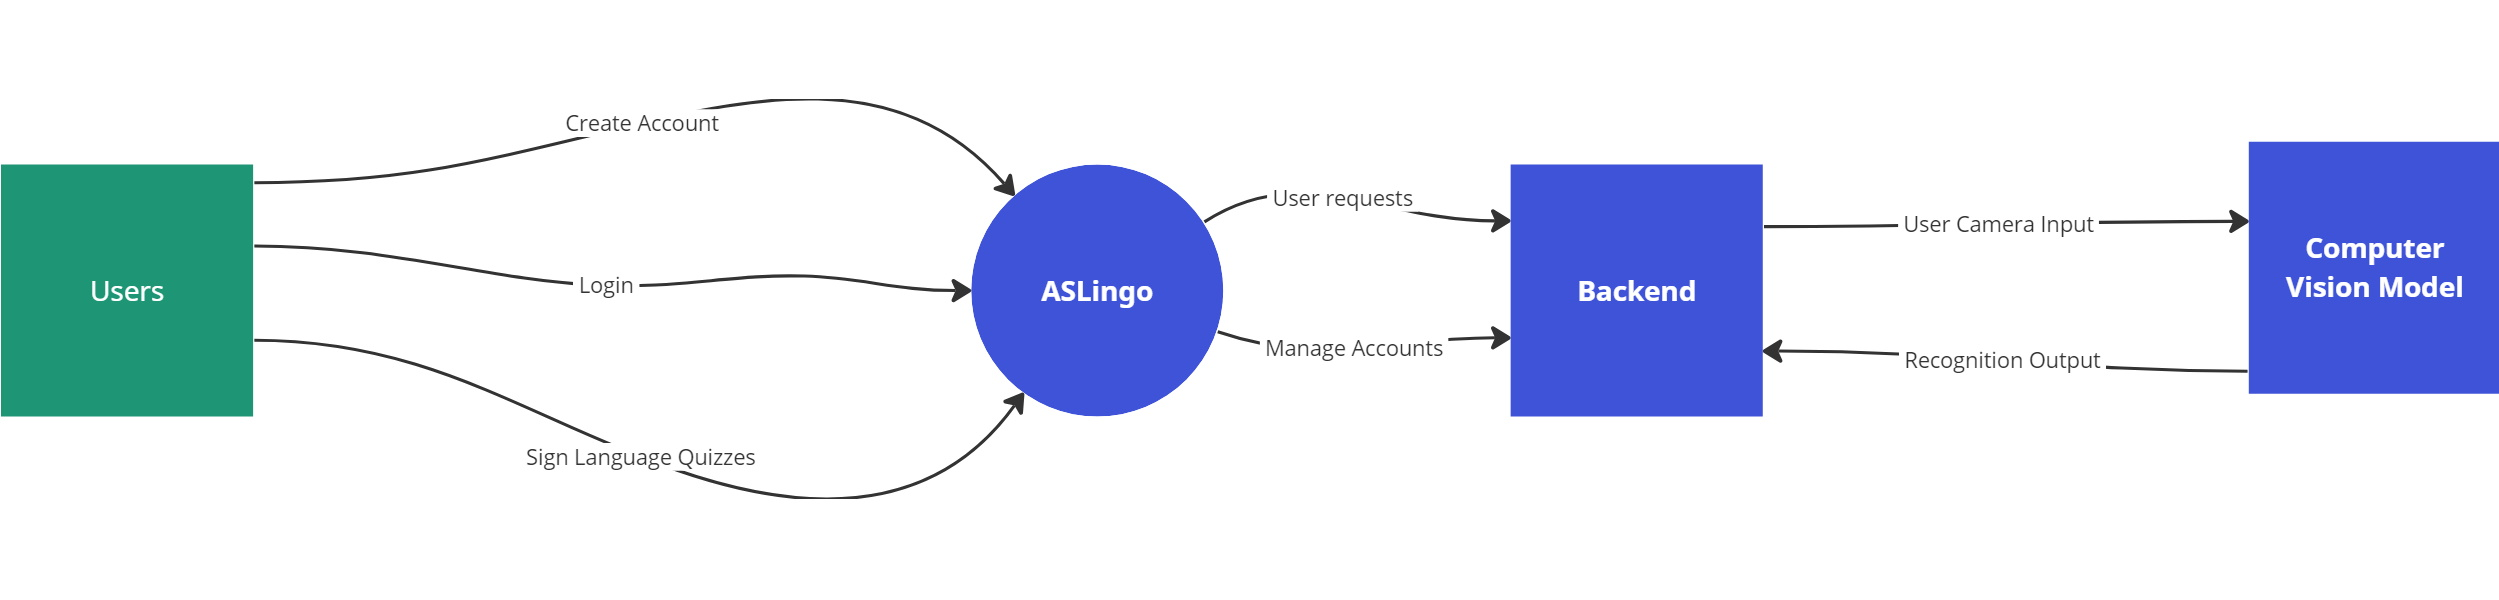
\includegraphics[scale=0.25]{context-diagram}
    \caption{Context Diagram}
\end{figure}

\subsubsection{Work Partitioning}

\begin{table}[H]
    \caption{Work Partitioning}
    \noindent \begin{tabularx}{\textwidth}{|c|p{0.2\linewidth}|X|X|}
    \hline 
    \textbf{Event ID} & \textbf{Event Name} &\textbf{Input and Output} & \textbf{Description}\\
    \hline
    1 & User login & User ID (in) \newline User Password (in) \newline Login Status (out) & User logs into the application, the system determines if login is successful. \\
    \hline
    2 & User logout & User ID (in) \newline Login Status (out) & User logs out of the application, system indicates whether log out is successful or not. \\
    \hline
    3 & User requests to start a test & User ID (in) & User starts a test. \\
    \hline
    4 & User signs through webcam & Camera Feed (in) \newline Recognized Sign (out) & User inputs sign language hand signs through webcam, the system responds with the corresponding sign output. \\
    \hline
    5 & User creates account & User ID (in) \newline User Email (in) \newline User Password (in) & User creates an account \\
    \hline
    6 & User checks learning progress & User ID (in) \newline User Progress (out) & User views account sign language learning progress. \\
    \hline
    7 & User completes a test & User ID (in) \newline User Score (in) & User completes a test with a given score. \\
    \hline
    \end{tabularx}
    \end{table}
  
  \subsubsection{Individual Product Use Cases}

  \begin{enumerate}
      \item 
      \textbf{Use Case Trigger:} User creates an account\\
      \textbf{Primary Actors:} user, ASLingo server\\
      \textbf{Outcomes:}
      \begin{enumerate}
          \item System creates an account with the designated username, password, and email
          \item System registers user as logged in
          \item System redirects user to home page
      \end{enumerate}

      \item
      \textbf{Use Case Trigger:} User logs into the application\\
      \textbf{Primary Actors:} user, ASLingo server\\
      \textbf{Outcomes:}
      \begin{enumerate}
          \item System checks if password matches for corresponding username
          \item System registers user as logged in
          \item System redirects user to home page
      \end{enumerate}
      
      \item
      \textbf{Use Case Trigger:} User logs out of the application\\
      \textbf{Primary Actors:} user, ASLingo server\\
      \textbf{Outcomes:}
      \begin{enumerate}
          \item System registers user as logged out
          \item System redirects user to login page
      \end{enumerate}

      \item
      \textbf{Use Case Trigger:} User requests to start a test\\
      \textbf{Primary Actors:} user, ASLingo server\\
      \textbf{Outcomes:}
      \begin{enumerate}
          \item System redirects user to testing page
          \item System requests to turn on user webcam
          \item System receives video data from user webcam
      \end{enumerate}

      \item
      \textbf{Use Case Trigger:} User signs through webcam\\
      \textbf{Primary Actors:} user, ASLingo server, ASLingo Computer Vision Model\\
      \textbf{Outcomes:}
      \begin{enumerate}
          \item System interprets user signs with computer vision model
          \item System responds informing user of correctness of sign
      \end{enumerate}

      \item
      \textbf{Use Case Trigger:} User checks learning progress\\
      \textbf{Primary Actors:} user, ASLingo server\\
      \textbf{Outcomes:}
      \begin{enumerate}
          \item System receives request from user to view learning progress
          \item System responds with user progress
      \end{enumerate}

      \item
      \textbf{Use Case Trigger:} User completes a test\\
      \textbf{Primary Actors}: user, ASLingo server\\
      \textbf{Outcomes:}
      \begin{enumerate}
          \item System registers that user completed test, and saves user score
      \end{enumerate}

      \item
      \textbf{Use Case Trigger:} User requests a new password\\
      \textbf{Primary Actors}: user, ASLingo server\\
      \textbf{Outcomes:}
      \begin{enumerate}
          \item System verifies email has a registered account
          \item System sends email with unique url to reset password to verified email
          \item System resets password to email and re-prompts sign in
      \end{enumerate}

\end{enumerate}

\subsubsection{Traceability Matrix}

\begin{table}[ht]
\centering
\resizebox{\textwidth}{!}{
\begin{tabular}{lllllllll}
                             & \multicolumn{8}{c}{Use Case No.}                                                                                                                                                                      \\ \cline{2-9} 
\multicolumn{1}{l|}{Req. No} & \multicolumn{1}{l|}{1} & \multicolumn{1}{l|}{2} & \multicolumn{1}{l|}{3} & \multicolumn{1}{l|}{4} & \multicolumn{1}{l|}{5} & \multicolumn{1}{l|}{6} & \multicolumn{1}{l|}{7} & \multicolumn{1}{l|}{8} \\ \hline
\multicolumn{1}{|l|}{0}      & \multicolumn{1}{l|}{}  & \multicolumn{1}{l|}{}  & \multicolumn{1}{l|}{}  & \multicolumn{1}{l|}{}  & \multicolumn{1}{l|}{}  & \multicolumn{1}{l|}{}  & \multicolumn{1}{l|}{}  & \multicolumn{1}{l|}{}  \\ \hline
\multicolumn{1}{|l|}{1}      & \multicolumn{1}{l|}{}  & \multicolumn{1}{l|}{}  & \multicolumn{1}{l|}{}  & \multicolumn{1}{l|}{X} & \multicolumn{1}{l|}{}  & \multicolumn{1}{l|}{}  & \multicolumn{1}{l|}{}  & \multicolumn{1}{l|}{}  \\ \hline
\multicolumn{1}{|l|}{2}      & \multicolumn{1}{l|}{}  & \multicolumn{1}{l|}{}  & \multicolumn{1}{l|}{}  & \multicolumn{1}{l|}{X} & \multicolumn{1}{l|}{}  & \multicolumn{1}{l|}{}  & \multicolumn{1}{l|}{}  & \multicolumn{1}{l|}{}  \\ \hline
\multicolumn{1}{|l|}{3}      & \multicolumn{1}{l|}{}  & \multicolumn{1}{l|}{}  & \multicolumn{1}{l|}{}  & \multicolumn{1}{l|}{}  & \multicolumn{1}{l|}{X} & \multicolumn{1}{l|}{}  & \multicolumn{1}{l|}{}  & \multicolumn{1}{l|}{}  \\ \hline
\multicolumn{1}{|l|}{4}      & \multicolumn{1}{l|}{X} & \multicolumn{1}{l|}{}  & \multicolumn{1}{l|}{}  & \multicolumn{1}{l|}{}  & \multicolumn{1}{l|}{}  & \multicolumn{1}{l|}{}  & \multicolumn{1}{l|}{}  & \multicolumn{1}{l|}{}  \\ \hline
\multicolumn{1}{|l|}{5}      & \multicolumn{1}{l|}{}  & \multicolumn{1}{l|}{X} & \multicolumn{1}{l|}{}  & \multicolumn{1}{l|}{}  & \multicolumn{1}{l|}{}  & \multicolumn{1}{l|}{}  & \multicolumn{1}{l|}{}  & \multicolumn{1}{l|}{}  \\ \hline
\multicolumn{1}{|l|}{6}      & \multicolumn{1}{l|}{}  & \multicolumn{1}{l|}{}  & \multicolumn{1}{l|}{}  & \multicolumn{1}{l|}{}  & \multicolumn{1}{l|}{X} & \multicolumn{1}{l|}{}  & \multicolumn{1}{l|}{}  & \multicolumn{1}{l|}{}  \\ \hline
\multicolumn{1}{|l|}{7}      & \multicolumn{1}{l|}{}  & \multicolumn{1}{l|}{}  & \multicolumn{1}{l|}{}  & \multicolumn{1}{l|}{}  & \multicolumn{1}{l|}{}  & \multicolumn{1}{l|}{X} & \multicolumn{1}{l|}{}  & \multicolumn{1}{l|}{}  \\ \hline
\multicolumn{1}{|l|}{8}      & \multicolumn{1}{l|}{X} & \multicolumn{1}{l|}{}  & \multicolumn{1}{l|}{}  & \multicolumn{1}{l|}{}  & \multicolumn{1}{l|}{}  & \multicolumn{1}{l|}{X} & \multicolumn{1}{l|}{}  & \multicolumn{1}{l|}{}  \\ \hline
\multicolumn{1}{|l|}{9}      & \multicolumn{1}{l|}{}  & \multicolumn{1}{l|}{}  & \multicolumn{1}{l|}{}  & \multicolumn{1}{l|}{}  & \multicolumn{1}{l|}{}  & \multicolumn{1}{l|}{X} & \multicolumn{1}{l|}{X} & \multicolumn{1}{l|}{}  \\ \hline
\multicolumn{1}{|l|}{10}     & \multicolumn{1}{l|}{}  & \multicolumn{1}{l|}{}  & \multicolumn{1}{l|}{}  & \multicolumn{1}{l|}{X} & \multicolumn{1}{l|}{}  & \multicolumn{1}{l|}{}  & \multicolumn{1}{l|}{}  & \multicolumn{1}{l|}{}  \\ \hline
\multicolumn{1}{|l|}{11}     & \multicolumn{1}{l|}{}  & \multicolumn{1}{l|}{}  & \multicolumn{1}{l|}{}  & \multicolumn{1}{l|}{X} & \multicolumn{1}{l|}{}  & \multicolumn{1}{l|}{}  & \multicolumn{1}{l|}{}  & \multicolumn{1}{l|}{}  \\ \hline
\multicolumn{1}{|l|}{12}     & \multicolumn{1}{l|}{}  & \multicolumn{1}{l|}{}  & \multicolumn{1}{l|}{X} & \multicolumn{1}{l|}{}  & \multicolumn{1}{l|}{}  & \multicolumn{1}{l|}{}  & \multicolumn{1}{l|}{}  & \multicolumn{1}{l|}{}  \\ \hline
\multicolumn{1}{|l|}{13}     & \multicolumn{1}{l|}{}  & \multicolumn{1}{l|}{}  & \multicolumn{1}{l|}{}  & \multicolumn{1}{l|}{}  & \multicolumn{1}{l|}{}  & \multicolumn{1}{l|}{}  & \multicolumn{1}{l|}{}  & \multicolumn{1}{l|}{X} \\ \hline
\end{tabular}}
\end{table}


\newpage

\subsection{Functional Requirements}

\begin{longtable}{| c | p{4cm}| p{6cm}|}
    \caption{Functional Requirements of ASLingo} \\
    \hline
    \textbf{Requirement No.} & \textbf{Description} &\textbf{Rationale}\\
    \hline
    FR1 & The system should be able to connect with a camera. & Connecting with a camera is a requirement for providing input to the system for hand sign recognition. \\
    \hline
    FR2 & The system should be able to recognize American Sign Language hand signs. & Hand sign recognition is a requirement for users to practice what they have been learning. \\
    \hline
    FR3 & The system should allow users to create an account. & Account creation is a requirement for users to save progression. \\
    \hline
    FR4 & The system should allow users to sign into their account if it exists. & Account sign-in is a requirement for users to save progression. \\
    \hline
    FR5 & The system should allow users to sign out of their account if they are signed into it. & Account sign-out is necessary for good account security practices. \\
    \hline
    FR6 & The system should provide a diagnostic quiz for new users. & A diagnostic quiz is a requirement for determining the current skill level of the user. \\
    \hline
    FR7 & The system should provide a progression-based course for ASL. & A progression-based course is a requirement for ensuring users are taught ASL in a comprehensive manner. \\
    \hline
    FR8 & The system should save user progress. & Saving user progress is a requirement for ensuring the user follows the progression-based course. \\
    \hline
    FR9 & The system should allow users to access the program via a web application & The system is being built for a web application, so the user should be able to access it in this way. \\
    \hline
    FR10 & The system should be able to communicate to the user if they have answered the prompt correctly. & The user should know if they have answered the prompt correctly to learn the language correctly. \\ 
    \hline
    FR11 & The system should notify the user of any potential errors that may arise during camera recognition. & This will let the user know if they need to adjust their input setting (camera angle, lighting etc.) so the system can accurately access their hand signs. \\
    \hline
    FR12 & The system should allow the user to their desired testing track from a selection of testing categories. & This is to provide variation in the manner of testing as well as in the subject matter that the user can test themselves on. \\
    \hline
    FR13 & The system should allow the user to reset their password to their registered account & Account security and accessibility are necessary for account use\\
    \bottomrule
\end{longtable}

\section{Non-Functional Requirements}

\subsection{Look and Feel Requirements}

\begin{table}[H]
\caption{Look and Feel Non-Functional Requirements}
\noindent \begin{tabular}{| c | p{3cm}| p{3cm}| p{3cm}|}
\hline 
\textbf{Requirement No.} & \textbf{Description} & \textbf{Rationale} & \textbf{Fit Criterion}\\
\hline
LFR1 & The system should remind users of similar language learning applications. & This will allow users to use the system intuitively if they have knowledge of other learning apps. & Ask a sample of users to rate how familiar/easy to use it is compared to other language learning apps. \\
\hline
LFR2 & The system should show the user how much progress they have made in their learning schedule. & The user should be able to gain feedback from the system about how much they learned. & The developers shall certify the product complies with these requirements by ensuring the user has a metric to understand their current progress. \\
% (level system, progress bar, score after a quiz etc.) 
\hline
LFR3 & The system should clearly show the user if they have answered the prompt correctly. & The user should gain feedback about if they are correct with the hand sign they have shown. & The developers shall certify the product shows the user the correct response based on their input. \\
\bottomrule
\end{tabular}
\end{table}

\subsection{Usability and Humanity Requirements}

\begin{table}[H]
\caption{Usability and Humanity Non-Functional Requirements}
\noindent \begin{tabular}{| c | p{3cm}| p{3cm}| p{3cm}|}
\hline 
\textbf{Requirement No.} & \textbf{Description} & \textbf{Rationale} & \textbf{Fit Criterion}\\
\hline
UHR1 & The system should be able to be used by people with little to no training. & The system should be able to be used without the need for formal training to make it easier for the average user. & After their first encounter with the product, 75\% of users shall report if they are comfortable using the application.\\
\hline
UHR2 & The system should be able to be used by people who are hard of hearing or deaf, as well as those who are able to hear. & The system should be accessible for all people wanting to learn ASL. & Users will be asked to rate their experience using the application on a scale of 1-10, with the average reporting a score above 7. \\
\hline
UHR3 & The system should allow users to personalize their account. & The user should be able to input their name, see their progress etc. & The developers shall certify the product complies with these requirements by ensuring the users will be able to do the required actions. \\
% (avatar, name, progress; personalization)
\hline
UHR4 & The system should show the user if the input needs to be adjusted. & The user should know if they need to change their camera angle, lighting etc. for the system to accurately give them proper feedback. & The developers shall certify the product complies with these requirements by ensuring the system gives user feedback where appropriate.\\
\bottomrule
\end{tabular}
\end{table}

\subsection{Performance Requirements}

\begin{table}[H]
\caption{Performance Non-Functional Requirements}
\noindent \begin{tabular}{| c | p{3cm}| p{3cm}| p{3cm}|}
\hline 
\textbf{Requirement No.} & \textbf{Description} & \textbf{Rationale} & \textbf{Fit Criterion}\\
\hline
PR1 & The system should respond to user input quickly. & If a user has to wait too long after an input they may be less engaged. & 95\% of tests should repond to user input within 1 second. \\
\hline
PR2 & The system should be able to accurately determine the sign shown by the user. & The system must be able to understand what hand signs the user is inputing to ensure they are learning effectively. & The system should accurately determine the correct hand sign from a user in 95\% of tests. \\
\bottomrule
\end{tabular}
\end{table}

\subsection{Operational and Environmental Requirements}

\begin{table}[H]
\caption{Operational and Environmental Non-Functional Requirements}
\noindent \begin{tabular}{| c | p{3cm}| p{3cm}| p{3cm}|}
\hline 
\textbf{Requirement No.} & \textbf{Description} & \textbf{Rationale} & \textbf{Fit Criterion}\\
\hline
OER1 & The system should be used as a web application on a browser/laptop. & The system is being built for a web application, so the user should be able to access it in this way. & 95\% of users are able to successfully use the product as a web application on a broswer source. \\
\hline
OER2 & The system should be able to access a user's camera device. & The user's camera will be used as the input device to see the user's hand signs. & 90\% of users are able to successfully use their camera on their input device. \\
\bottomrule
\end{tabular}
\end{table}

\subsection{Maintainability and Support Requirements}

\begin{longtable}{| c | p{3cm}| p{3cm}| p{3cm}|}
\caption{Maintainability and Support Non-Functional Requirements} \\
\hline 
\textbf{Requirement No.} & \textbf{Description} & \textbf{Rationale} & \textbf{Fit Criterion}\\
\hline
MSR1 & The system should be tested regularly to ensure it's functionality and usability. & This will ensure that the system does not experience any bugs or other errors when being updated over time. & The product must pass 95\% of its developer tests at least once a week. \\
\hline
MSR2 & The code implemented in the system should adhere to specified coding standards to ensure its readabilty for future updates. & This will ensure that the system code can be understood over time to ensure readability and maintainability for future updates. & The developers shall certify the product complies with these requirements by adhering to the coding standards specified in our Development Plan, and will be certified through a peer review process. \\
\hline
MSR3 & The code implemented in the system should be tested using code coverage methods to test all functions of the system. & This will ensure that all aspects of the system can be tested for errors, and fixed if errors are found during testing. & 80\% of code coverage shall be achieved when running test cases on the system. \\
\hline
MSR4 & The system should allow for new signs to be added over the lifespan of the system. & This will allow the system to expand over time, as well as be able to add in new modern signs. The modules of the product will be written according to coding standards to allow for new additions to the system. & The developers shall certify the product complies with these requirements by adhering to coding standards and ensuring readability for future developers. \\
\bottomrule
\end{longtable}

\subsection{Security Requirements}

\begin{table}[H]
\caption{Security Non-Functional Requirements}
\noindent \begin{tabular}{| c | p{3cm}| p{3cm}| p{3cm}|}
\hline 
\textbf{Requirement No.} & \textbf{Description} & \textbf{Rationale} & \textbf{Fit Criterion}\\
\hline
SR1 & The system should allow the user to access their account after creating it. & The user should be able to create an account and be able to log in and out of it as needed. & The developers shall certify the product complies with these requirements by ensuring the user can log in and out. \\
\hline
SR2 & The system should ensure that the system is trained on correct information. & The system should not be trained using incorrect usage of ASL as this would contradict the goal of learning how to use the language properly. & The developers shall certify the product complies with these requirements by selecting trusted data sources and verifying the credibility of input data. \\
\hline
SR3 & The system should store user account information using encryption. & This will ensure that all user information will be kept private and secure. & The developers shall certify the product complies with these requirements by ensuring encryption is used in the system. \\
\bottomrule
\end{tabular}
\end{table}

\subsection{Cultural Requirements}

\begin{table}[H]
\caption{Cultural Non-Functional Requirements}
\noindent \begin{tabular}{| c | p{3cm}| p{3cm}| p{3cm}|}
\hline 
\textbf{Requirement No.} & \textbf{Description} & \textbf{Rationale} & \textbf{Fit Criterion}\\
\hline
CR1 & The system should be written in Canadian English and teach users using American Sign Language. & The primary users of this application at this stage will be Canadian English speakers who want to learn American Sign Language. & The developers shall certify the product complies with these requirements by adhering to Canadian English and American Sign Language standards. \\
\bottomrule
\end{tabular}
\end{table}

\subsection{Legal Requirements}

\begin{table}[H]
\caption{Legal Non-Functional Requirements}
\noindent \begin{tabular}{| c | p{3cm}| p{3cm}| p{3cm}|}
\hline 
\textbf{Requirement No.} & \textbf{Description} & \textbf{Rationale} & \textbf{Fit Criterion}\\
\hline
LR1 & The system should adhere to Canadian user privacy laws. &  The system should never share user information, and should ensure user's data is kept private and secure. & The developers shall certify the product complies with the Canadian Personal Information Protection and Electronic Documents Act (PIPEDA) to ensure user's data safety. \\
\hline
LR2 & The system should not train the model on personal/confidential/illegal data & The system should only be trained on data that is safe to use, and is in the public domain. & The developers shall certify the product complies with these requirements by selecting trusted data sources and verifying the credibility of input data. \\
\bottomrule
\end{tabular}
\end{table}

\subsection{Health and Safety Requirements}

\begin{table}[H]
\caption{Health and Safety Non-Functional Requirements}
\noindent \begin{tabular}{| c | p{3cm}| p{3cm}| p{3cm}|}
\hline 
\textbf{Requirement No.} & \textbf{Description} & \textbf{Rationale} & \textbf{Fit Criterion}\\
\hline
HSR1 & The system should warn users to ensure they have enough space to practice ASL in their environment. & This will ensure that the user will not use this application if there is not enough space to comfortably do so. & The developers shall certify the product complies with these requirements by ensuring the system warns the user appropriately. \\
\bottomrule
\end{tabular}
\end{table}

\section{Project Issues}

\subsection{Open Issues}
There are currently no open issues with the project at the moment.

\subsection{Off-the-Shelf Solutions}
\begin{enumerate}
    \item The ASL App is a mobile exclusive platform with 2,500+ signs and phrases to teach ASL via short video clips. This app offers 4 packs for free with the basics like the alphabet, numbers, and universal gestures. Paid packs are also available ex. compliments, moods, and social gestures for \$0.99. The app ultimately serves as a mobile hub for common expressions to study and learn wherever you are.
    \item Canadian Hearing Services offer both in-person and virtual educational ASL courses for a variety of experience levels. These courses educate via teacher instruction, role play, videos, and work books. A variety of other public, private, and educational institutes offer similar courses and instructional content.
    \item Duolingo is a popular mobile application that provides language courses for many languages from across the world, with 50+ million monthly active users. The app utilizes gamification to encourage consistent user progress and interest. Majority of the courses are based on testing users on vocabulary and grammar via reading, listening, and speaking problems which increase in difficulty as users progress. Its courses are well developed through research and accord with global language standards, such as the Common European Framework of Reference for Languages (CEFR).
\end{enumerate}

\subsection{New Problems}
There are currently no new problems.

\subsection{Tasks}
\begin{itemize}
    \item Development should follow the agile methodology, with emphasis on different aspects of the project: front-end, back-end, and computer vision.
\end{itemize}

\subsection{Migration to the New Product}
Not applicable for our project.

\subsection{Risks}

\begin{enumerate}
    \item The primary risk of this product is the potential for error when trying to analyze and recognize a user's sign to give feedback or determine if their form is correct. This could cause users to improperly learn signs and hinder their learning.
\end{enumerate}

\subsection{Costs}
\begin{enumerate}
    \item Website domain - TBA
    \item App hosting platform - TBA
    \item Database - TBA
\end{enumerate}

\subsection{User Documentation and Training}
The system and its interface should be intuitive enough to learn how to use the app. User documentation to be supplied with the product should include a general setup guide and can include a glossary for basic signs, such as for the alphabet.

\subsection{Waiting Room}
\begin{enumerate}
    \item The system should incorporate full body signs (eg. the sign for "shorts") and facial expression/body language recognition, as they are a crucial aspect of sign language.
    \item The system should provide different courses for learners of varying skill level.
    \item The system should teach other common sign languages.
\end{enumerate}

\subsection{Ideas for Solutions}

N/A

\newpage

%\subsection{Symbolic Parameters}

\section{Appendix --- Reflection}

%The information in this section will be used to evaluate the team members on the
%graduate attribute of Lifelong Learning.  Please answer the following questions:

%\begin{enumerate}
%  \item Which of the courses you have taken, or are currently taking, will help
%  your team to be successful with your capstone project.
%  \item What knowledge and skills will the team collectively need to acquire to
%  successfully complete this capstone project?  Examples of possible knowledge
%  to acquire include domain specific knowledge from the domain of your
%  application, or software engineering knowledge, mechatronics knowledge or
%  computer science knowledge.  Skills may be related to technology, or writing,
%  or presentation, or team management, etc.  You should look to identify at
%  least one item for each team member.
%  \item For each of the knowledge areas and skills identified in the previous
%  question, what are at least two approaches to acquiring the knowledge or
%  mastering the skill?  Of the identified approaches, which will each team
%  member pursue, and why did they make this choice?
%\end{enumerate}

\begin{enumerate}
    \item Many software design and principles courses contribute to the team's success on the capstone project. Our project is primarily software-based, involving a combination of everything taught throughout the program, including software design, development, and documentation. Here is a list of specific courses that were particularly helpful for us: 
    \begin{itemize}
        \item SFWRENG 2AA4
        \item SFWRENG 2C03
        \item SFWRENG 2XA3
        \item SFWRENG 2XB3
        \item SFWRENG 3A04
        \item SFWRENG 3RA3
        \item SFWRENG 3S03
        \item SFWRENG 3XA3
        \item SFWRENG 4HC3
    \end{itemize}
    \item Some overall knowledge and skills that will be required in the entire team include domain knowledge (the fundamentals of ASL and basic signing), skills in technical tools for development (React, OpenCV, Python, etc.), documentation writing skills, and communication skills for connecting with stakeholders.
    \begin{itemize}
        \item Edward -- On the technical side, I will need to familiarize myself with OpenCV and computer vision in general. As well, I will need to learn how to apply machine learning to recognizing specific hand motions. On the non-technical side, I will need to familiarize myself with ASL and at minimum learn basic hand signs. I aim to learn more than just the fundamentals, so I can help to design the course that our project provides.
	    \item Cassidy -- For technical skills, I am mostly familiar with back end development, so through this project I hope to learn more about front end web development, as well as learning some fundamentals of machine learning for the hand motions. I also hope to be able to learn some ASL through this project, as well as further develop project development and time management skills.
        \item Stanley -- As I would like to familiarize myself with computer vision, I will also need to focus on some back-end fundamentals as well. Although I'll be focusing mainly on the front-end, since our computer vision component will work hand and hand with the back-end of ASLingo, I'll naturally need to be able to know both at a basic level. For non-technical skills, I'd like to gain more experience in communicating with stakeholders on a more project management level.
        \item Jeremy -- With a focus on the full stack development role within the team I will have to become comfortable with modern full stack development technologies and practises. Such practises will include creating a responsive front end that allows for an intuitive user experience, creating a back end ecosystem to store our data, and integrating the OpenCV and ML aspects. I also look forward to using github CI/CD and ensuring good code coverage testing and smooth deployments for future changes.
        \item Andrew -- I aim to bring my industry experience in the field of system verification and translate that over to this project.  I'll mainly be focusing on ensuring correctness within the python-OPenCV back-end by writing units tests to ensure complete code coverage.  Naturally this will require me to understand OpenCV enough to test for edge cases and more niche scenarios in which we do not intend for the project to be used while working in lock-step with the rest of the team. I hope to additionally polish up on my communications and UI design skills to bring forward a design that will satisfy the stakeholders and make the use of our final product as smooth as possible.
    \end{itemize}
    \item All team members are making it a personal goal to attend as many McMaster Sign Language Club meetings as possible to learn basic signs and gestures, as well as interact with some of our stakeholders. To learn full stack development we will be following tutorials and best practises from the industry standards such as Mozilla MDN Web Docs, documentation from our framework and language of choice,and articles posted on FreeCodeCamp, GeeksForGeeks, Medium etc. Learning OpenCV and AI/ML topics will also be learned via a similar method. 
    
\end{enumerate}


\end{document}